\documentclass[a4paper]{article}

\usepackage{scrextend}
\changefontsizes{13pt}
\usepackage[utf8]{vietnam}
\usepackage[T5]{fontenc}
\usepackage{times}
\usepackage{amsmath,amssymb}
\usepackage{siunitx}
\usepackage{booktabs}
\usepackage{geometry}
\usepackage[hypertexnames=false]{hyperref}
\usepackage{graphicx}
\usepackage{float}
\usepackage{titlesec}
\usepackage{xcolor}
\usepackage{listings}

\geometry{margin=2cm}
\hypersetup{
  colorlinks=true,
  linkcolor=blue,
  urlcolor=blue,
  citecolor=blue
}

\renewcommand{\today}{%
  \ifnum\day<10 0\fi\the\day/\ifnum\month<10 0\fi\the\month/\the\year}

\titleformat{\section}{\bfseries\normalsize}{\thesection}{0.6em}{}
\titleformat{\subsection}{\bfseries\normalsize}{\thesubsection}{0.6em}{}
\titleformat{\paragraph}{\bfseries\normalsize}{\theparagraph}{0.6em}{}
\titlespacing*{\section}{0pt}{0.8\baselineskip}{0.4\baselineskip}
\titlespacing*{\subsection}{0pt}{0.6\baselineskip}{0.3\baselineskip}
\titlespacing*{\paragraph}{0pt}{0.4\baselineskip}{0.2\baselineskip}

\lstdefinestyle{py}{
  basicstyle=\ttfamily\normalsize,
  numbers=left,
  numberstyle=\normalsize\color{gray},
  stepnumber=1,
  numbersep=10pt,
  frame=single,
  breaklines=true,
  showstringspaces=false,
  tabsize=2,
}

\begin{document}
\begin{center}
{\LARGE\bfseries BÀI TẬP NHẬN DẠNG ĐỐI TƯỢNG}\par
\vspace{0.5\baselineskip}
Nhóm 1: \par
Vũ Đức Minh -- 20250109E\par
Phạm Ngọc Hà -- 20214654\par
\vspace{0.5\baselineskip}
\today
\end{center}
\vspace{\baselineskip}

\section{Đề bài}
Từ hình \texttt{hàm.png}, đối tượng bậc cao được cho dưới dạng hàm truyền có trễ:

\begin{figure}[H]
\centering
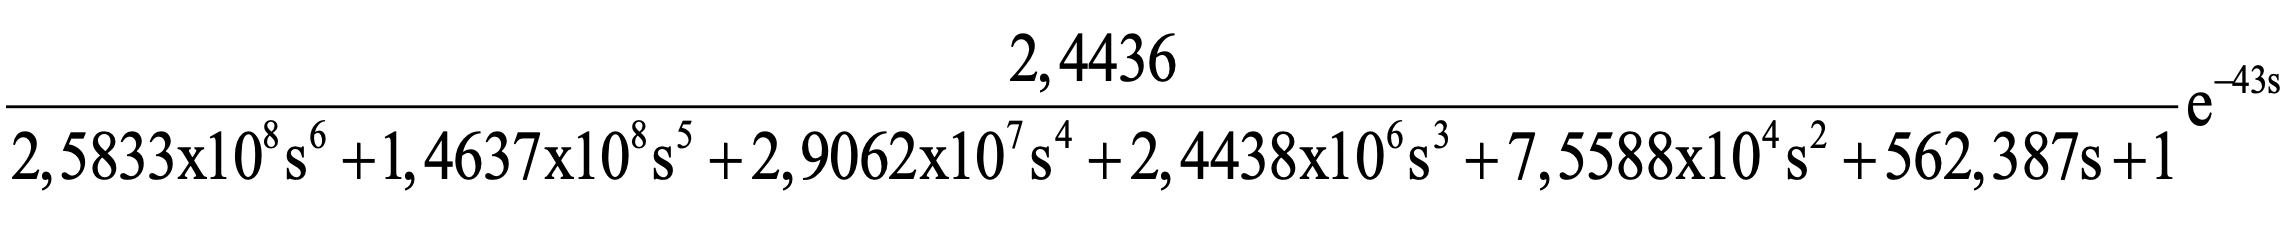
\includegraphics[width=0.92\textwidth]{hàm.png}
\caption{Hàm truyền đối tượng bậc cao và dạng xấp xỉ SOPDT tham khảo.}
\label{fig:ham-truyen}
\end{figure}

\section{Mục tiêu nhận dạng SOPDT}
Mục tiêu là nhận dạng một mô hình SOPDT (bậc hai có trễ) sao cho đáp ứng bậc thang xấp xỉ tốt đáp ứng của \(G(s)\):
\[
\hat{G}(s)=\frac{K}{(1+T_1 s)(1+T_2 s)}e^{-Ls},
\qquad K>0,\; T_1>0,\;T_2>0,\;L\ge 0.
\]

\section{Mô phỏng đặc tính quá độ từ hàm truyền bậc cao}
\subsection{Xấp xỉ trễ bằng Padé}
Thành phần trễ \(e^{-43s}\) được xấp xỉ bằng Padé đối xứng \([n/n]\) (trong mã sử dụng \(n=8\)) để thu được một hàm truyền hữu tỉ, thuận lợi cho mô phỏng trong miền Laplace.

\subsection{Tính đáp ứng bậc thang}
Đáp ứng bậc thang \(y(t)\) được tính từ
\[
Y(s)=\frac{G(s)}{s},
\]
và khai triển thành tổng các phần tử thặng dư:
\[
y(t)=\sum_i r_i e^{p_i t},
\]
trong đó \(p_i\) là các cực của \(Y(s)\), \(r_i\) là thặng dư tương ứng. (Trong thực nghiệm chạy mã, các phần ảo phát sinh do sai số số học rất nhỏ và được lấy phần thực.)

\begin{figure}[H]
\centering
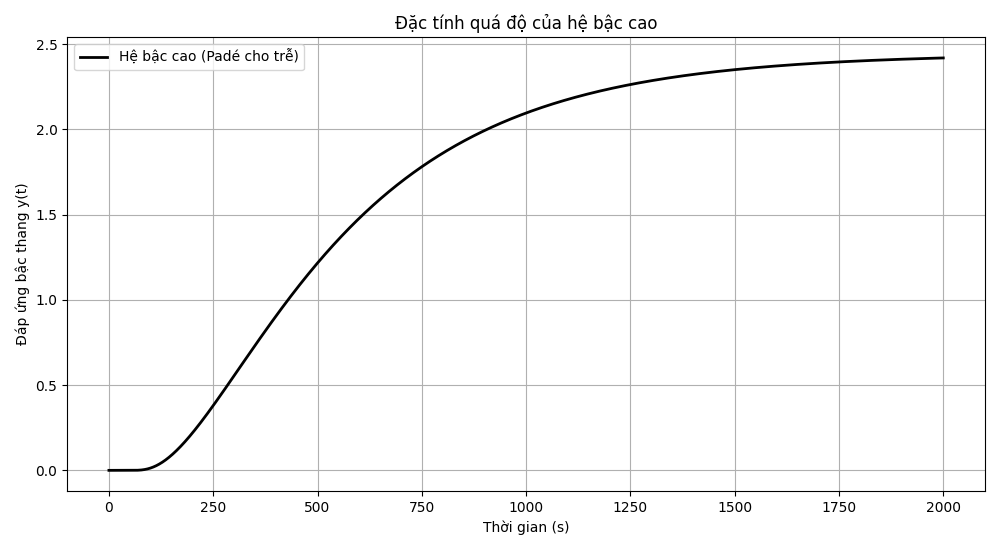
\includegraphics[width=0.92\textwidth]{dac-tinh-he-bac-cao.png}
\caption{Đặc tính quá độ của hệ bậc cao}
\label{fig:dac-tinh-he-bac-cao}
\end{figure}

\section{Nhận dạng tham số SOPDT}
\subsection{Tiêu chuẩn tối ưu}
Tham số \((K,T_1,T_2,L)\) được chọn sao cho sai số bình phương tối thiểu giữa đáp ứng bậc thang của hệ bậc cao và đáp ứng bậc thang của mô hình SOPDT là nhỏ nhất. Chỉ tiêu sai số báo cáo là
\[
\mathrm{RMSE}=\sqrt{\frac{1}{N}\sum_{i=1}^{N} (y_i-\hat{y}_i)^2 }.
\]

\subsection{Chiến lược tìm kiếm tham số}
Do mục tiêu chính là xấp xỉ đáp ứng, nhóm dùng \textbf{grid search} trên \((T_1,T_2,L)\) (với \(T_2\ge T_1\)). Với mỗi bộ \((T_1,T_2,L)\), hệ số khuếch đại \(K\) được tính tối ưu theo bình phương tối thiểu tuyến tính:
\[
K^\star=\arg\min_{K}\sum_{i=1}^{N}\bigl(y_i-K\,s(t_i;T_1,T_2,L)\bigr)^2
=\frac{\langle y, s\rangle}{\langle s,s\rangle},
\]
với \(s(t;T_1,T_2,L)\) là đáp ứng bậc thang chuẩn hoá của khối \(\frac{1}{(1+T_1 s)(1+T_2 s)}e^{-Ls}\).

\subsection{Kết quả nhận dạng}
Chạy chương trình \texttt{draft.py} thu được mô hình SOPDT:
\[
K = 2.431920,\quad
T_1 = 168.351708,\quad
T_2 = 353.566562,\quad
L = 75.949367,
\]
với \(\mathrm{RMSE}=3.706710\times 10^{-3}\).

Phương trình xấp xỉ:
\[
\hat{G}(s)=\frac{2.431920}{(1+168.351708\,s)(1+353.566562\,s)}e^{-75.949367s}.
\]

\begin{figure}[H]
\centering
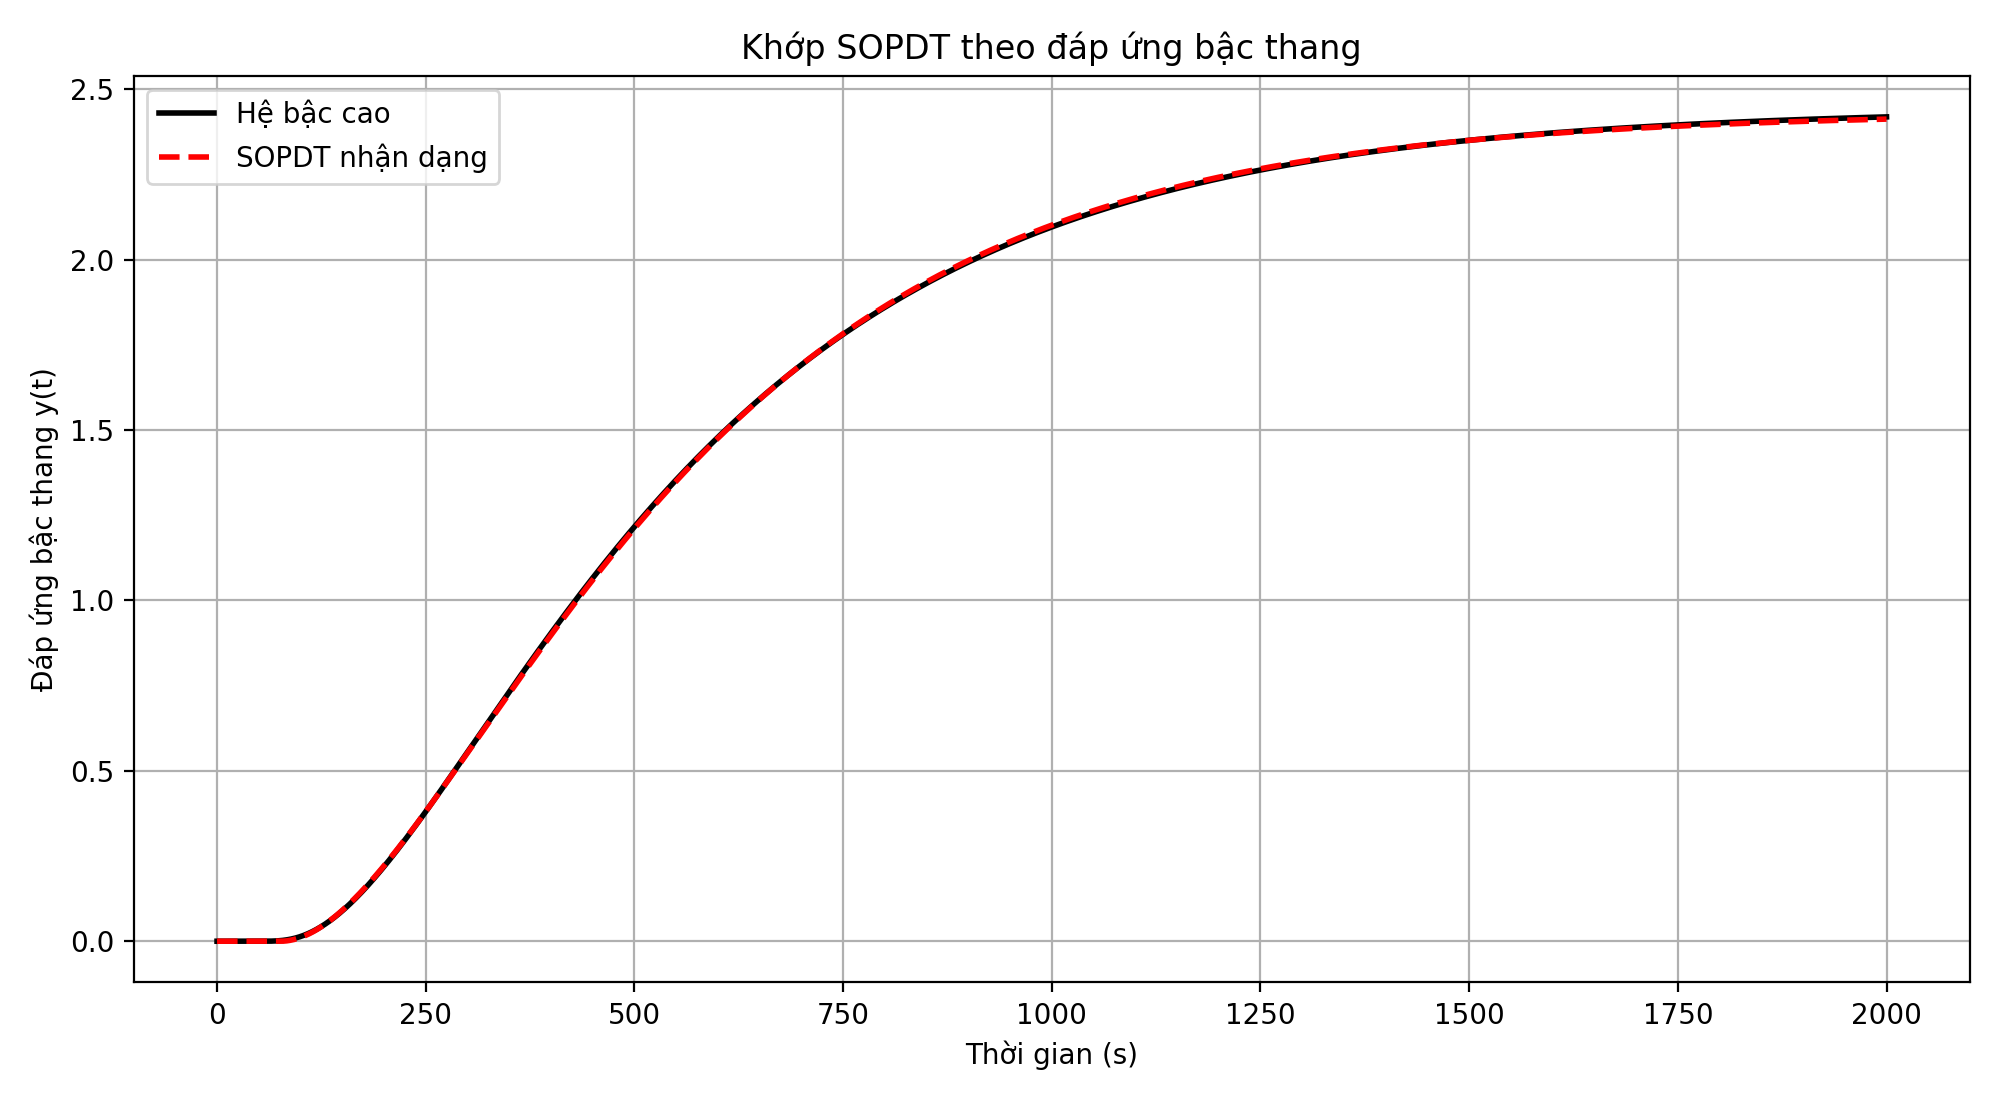
\includegraphics[width=0.92\textwidth]{khep-sopdt.png}
\caption{So sánh đáp ứng bậc thang của hệ bậc cao và mô hình SOPDT nhận dạng.}
\label{fig:khep-sopdt}
\end{figure}

\section{Nhận xét}
Mô hình SOPDT thu được tái hiện tốt dạng cong của đáp ứng bậc thang và thể hiện rõ thành phần trễ \(L\). Sai khác còn lại chủ yếu đến từ việc xấp xỉ trễ bằng Padé và giới hạn của cấu trúc SOPDT khi xấp xỉ hệ bậc cao.

\end{document}
